% All contribution chapters should follow a similar structure, with a
% mini-introduction and overview at the beginning and a conclusion at the
% end bookmarking a structured presentation of the contribution. This can be
% largely based on your publications.

\chapter{Modelo Base}\label{chap:modelo}
\section{Introducción}\label{sec:modelo:intro}
Ya teniendo en cuenta las dinámicas de los glóbulos rojos en el cuerpo humano, se procederá a analizar y simular el modelo matemático de estas propuesto por Eldestein en \cite{edelstein2005} y las técnicas de solución correspondientes. 

Es importante tener en cuenta que el modelo que sea que se analice debe tener concordancia con la vida real en cuanto a las variables y a las constantes utilizadas. La homeostasis es fundamental en todo proceso biológico y es por eso que el modelo y las simulaciones deben reflejar correctamente el equilibrio del sistema. Adicionalmente, es clave considerar que es imposible lograr una formulación matemática que este totalmente en concordancia con todos los procesos biológicos que suceden dentro del cuerpo humano, pues se debería tener en consideración una enorme cantidad de variables, de actores y de estados que se salen del propósito básico de simplificar el problema. De esta manera, los modelos propuestos son un acercamiento aproximado a la realidad del problema.

\section{Presentación del Modelo}\label{sec:modelo:presentacion}

Considerando la eliminación de glóbulos rojos por parte del bazo y su producción por la médula ósea para mantener la homeostasis y el diagrama compartimental de la figura \ref{sec:RBC:fig:VidaRBC}, el modelo propuesto por Eldestein es el siguiente:

$$R(n+1)=(1-f)R(n)+M(n),$$
$$M(n+1)=\gamma \cdot f\cdot R(n),$$

en donde $R=R(n)$ representa la cantidad de glóbulos rojos en el torrente sanguíneo en el $n$-ésimo día y $M=M(n)$ la cantidad de glóbulos rojos producidos por la médula ósea en el $n$-ésimo día. El parámetro $\gamma>0$ representa la cantidad de glóbulos rojos producida por cada uno eliminado y $0\leq f \leq 1$ es la fracción de glóbulos rojos que elimina el bazo cada día. Ni $\gamma$ ni $f$ tienen unidades dadas estas definiciones.

De esta manera, el modelo se puede interpretar de la siguiente manera: la cantidad de RBC's en el día $n+1$-ésimo, $R(n+1)$, es la fracción restante del día $n$-ésimo más lo que haya producido la médula ósea en el día $n$-ésimo; mientras que la cantidad de eritrocitos producidos por la médula ósea en el día $n+1$-ésimo, $M(n+1)$, es un múltiplo de la cantidad de glóbulos rojos eliminada en el día $n$-ésimo. Este modelo es una simplificación bastante acertada de lo visto en la figura \ref{sec:RBC:fig:VidaRBC} en cuanto a la relación entre producción y eliminación de RBC's. Es claro que, para ser aún más acertados, se podrían agregar muchas otras variables como el funcionamiento de los riñones para la producción de eritropoyetina, el proceso de absorción del hierro o la edad y estado de salud del sujeto analizado, pero estos complican innecesariamente el modelo y su análisis.

\section{Análisis del Modelo}\label{sec:modelo:analisis}

Ahora se procederá a analizar las soluciones del modelo a través de los métodos de ecuaciones en diferencias y de la matriz resultante del modelo.

\subsection{Método mediante Ecuaciones en Diferencias}

Nótese que las ecuaciones del modelo se pueden reducir a una única ecuación en términos de $R(n)$ de la siguiente manera:
$$M(n)=\gamma f R(n-1)$$
$$\implies R(n+1)=(1-f)R(n)+\gamma f R(n-1)$$
$$\implies R(n+2)=(1-f)R(n+1)+\gamma f R(n)$$
$$\implies R(n+2)-(1-f)R(n+1)-\gamma f R(n)=0.$$

Esta ecuación se puede tomar como una ecuación en diferencias homogénea lineal de grado 2, por lo que se pueden hallar sus soluciones al encontrar las raíces del polinomio característico de la ecuación:
$$p(\lambda)=\lambda^2-(1-f)\lambda-\gamma f$$
$$\implies \lambda_{1,2}=\dfrac{(1-f)\pm\sqrt{(1-f)^2+4\gamma f}}{2}.$$

Dado que $0\leq f \leq 1$ y $\gamma > 0$, entonces el radicando siempre será positivo, por lo que los valores $\lambda_{i}$ son números reales. De esta manera la solución general de la ecuación en diferencias es de la forma:
$$R(n)=c_1 \lambda_1^n+ c_2 \lambda_2^n,$$
$$M(n)=\gamma \cdot f R(n-1)= \gamma \cdot f(c_1 \lambda_1^{n-1}+ c_2 \lambda_2^{n-1})$$
$$\implies M(n)=c_3 \lambda_1^{n-1}+ c_4 \lambda_2^{n-1},$$
$$c3 = c_1\cdot \gamma \cdot f,$$
$$c4 = c_2\cdot \gamma \cdot f,$$

en donde $c_{i}$ ($i=1,2,3,4$) dependerán de las condiciones iniciales que se utilicen y los valores de cada parámetro.

\subsection{Método mediante Matrices}

La matriz resultante del modelo es:
$$X_{n+1}=\begin{pmatrix}
    R(n+1) \\
    M(n+1) 
    \end{pmatrix}=
    \begin{pmatrix}
    1-f & 1\\
    \gamma f & 0 
    \end{pmatrix} \cdot 
    \begin{pmatrix}
    R(n) \\
    M(n) \\
    \end{pmatrix}=
    \begin{pmatrix}
        1-f & 1\\
        \gamma f & 0 
        \end{pmatrix} X_n,$$

por lo que para el análisis de soluciones se debe estudiar la matriz
$$A=\begin{pmatrix}
    1-f & 1\\
    \gamma f & 0 
    \end{pmatrix}.$$

Los valores propios de $A$ se obtienen al calcular las soluciones $\lambda_{1,2}$ del determinante de $A-\lambda I$:
$$det(A-\lambda I) = \begin{vmatrix}
    1-f-\lambda & 1\\
    \gamma f & -\lambda 
    \end{vmatrix} = -\lambda(1-f-\lambda)-\gamma f$$

$$=\lambda^2-(1-f)\lambda-\gamma f,$$

utilizando la fórmula cuadrática, se obtiene
$$\lambda_{1,2}=\dfrac{(1-f)\pm\sqrt{(1-f)^2+4\gamma f}}{2}.$$

Los vectores propios correspondientes a estos valores propios son los vectores $\mathbf{v_{1,2}}$ que solucionan la ecuación
$$(A-\lambda_i I)\mathbf{v_i}=0, \:\:\: i=1,2,$$

y de esta manera la solución general del problema estará dada por

$$\begin{pmatrix}
    R(n) \\
    M(n) 
    \end{pmatrix}= (\lambda_1)^n \mathbf{v_1}+(\lambda_2)^n \mathbf{v_2}.$$


Nótese que ambos métodos, al tener el mismo polinomio característico, obtienen la misma solución general del sistema, esto implica que el modelo propuesto está bien fundamentado matemáticamente.


\section{Derivación de Parámetros y Análisis}\label{sec:modelo:parametros}

Los \textbf{equilibrios} de una ecuación en diferencias $x_n=f(x_{n-1},...,x_0)$ son los valores $x_n=x^*$ tales que $x^*=f(x^*,...,x^*)$. Considerando la ecuación en diferencias de una sola variable 
$$R(n+2)-(1-f)R(n+1)-\gamma f R(n)=0,$$
entonces si $x^*$ es un equilibrio, se debe cumplir que:
$$x^*-(1-f)x^*-\gamma f x^*=0$$
$$\implies x^*(1-(1-f)-\gamma\cdot f)=0,$$
$$\implies x^*(f-\gamma\cdot f)=0.$$

De esta manera, $x^*=0$ es un equilibrio del sistema, pero, adicionalmente, dado que $f$ es un valor fijo (como se verá más adelante) entonces también hay equilibrios en el sistema cuando $\gamma = 1$. Es decir que, para este valor del parámetro, cualquier valor de $R,M$ presenta un equilibrio. 

Para poder pasar a valores específicos de las soluciones encontradas, es necesario dar valores numéricos a los parámetros $\lambda$ y $f$, pues el modelo depende de estos y, junto a las condiciones iniciales, determinan las soluciones del problema. Para hallar estos parámetros, se utilizará la información brindada en la sección \ref{sec:RBC:vida} sobre la producción de glóbulos rojos a través de la médula ósea y de su eliminación por medio del bazo.

Inicialmente, es necesario declarar las condiciones iniciales del problema. Dado que las soluciones encontradas dependen, en el caso de ecuaciones en diferencias, de dos constantes o, en el caso de matrices, de dos vectores, es necesario que hayan dos condiciones iniciales del problema: $R(0)$ y $M(0)$ o $X_0$. $R(0)$ representa la cantidad de glóbulos rojos al momento inicial de la medida, que se tomará como 125 trillones ($25\times 10^{12}$). Para el caso de la matriz, se puede tomar que $R(0)$ se mantiene como en el caso anterior y tomar $M(0)=f\cdot R(0)$ pues el instante que se inicia la medición el paciente está totalmente sano y tiene el equilibrio en $\gamma = 1$. 

Ahora, determinar $f$ es relativamente sencillo, pues es el porcentaje diario de RBC's que elimina el cuerpo. Contando con que la cantidad promedio es de eritrocitos es de $25\times 10^{12}$ y que diariamente mueren $208\times 10^{9}$, entonces el porcentaje de glóbulos rojos eliminados diariamente por el bazo es del $0.832\%$, es decir que se puede tomar $f=0.00832$. 

Determinar el valor biológico de $\gamma$ es mucho más complicado, pues no ha sido posible determinar la cantidad de glóbulos rojos que produce una célula madre durante la eritropoyesis. Para hallar un valor adecuado de $\gamma$, se hará el análisis matemático y de las simulaciones con los valores ya establecidos. En todo caso, se puede hace el análisis para los diferentes casos:
\begin{enumerate}
    \item  $\gamma<1$: Este caso implica que el cuerpo produce una menor cantidad de eritrocitos respecto a la que elimina, por lo que los resultados deberían mostrar una caída en la cantidad de glóbulos rojos.
    \item $\gamma=1$: Este caso implica que el cuerpo produce la misma cantidad de eritrocitos respecto a la que elimina, por lo que los resultados deberían mostrar una estabilidad en la cantidad de glóbulos rojos.
    \item  $\gamma>1$: Este caso implica que el cuerpo produce una mayor cantidad de eritrocitos respecto a la que elimina, por lo que los resultados deberían mostrar un crecimiento en la cantidad de glóbulos rojos.
\end{enumerate}

En el caso esperado, es decir en el que el cuerpo alcanza la homeostasis, el valor deseado de $\gamma$ es $1$, pues de esta manera el cuerpo no pierde células, ya que todas aquellas que mueren son producidas. En todo caso, las simulaciones que se hagan utilizarán variaciones en este parámetro con valores cualquiera de ejemplo que puedan ilustrar el análisis.

Como ya se ha visto en la sección \ref{sec:modelo:analisis}, las soluciones del problema dependen de las constantes y de los valores iniciales, a continuación se calcularán las soluciones bajo los valores derivados para cada parámetro: $\gamma = 1$, $f = 0.00832$, $R(0)=25\times 10^{12}$, $M(0)=208\times 10^{9}$ 

\begin{itemize}
    \item Para el caso de ecuaciones en diferencias, se obtiene que las soluciones del polinomio característico de la ecuación son:
        $$\lambda_{1,2}=\dfrac{(1-f)\pm\sqrt{(1-f)^2+4\gamma f}}{2}$$
        $$=\dfrac{(1-0.00832)\pm \sqrt{(1-0.00832)^2+4(0.00832)}}{2}$$
        $$\implies \lambda_1 = 1,\;\;\; \lambda_2 = -0.00832=-f.$$
        Y así, la solución general está dada por 
        $$R(n)=c_1+c_2(-0.00832)^n$$
        $$R(0)=25\times 10^{12}=c_1+c_2$$
        $$R(1)=(1-f)R(0)+M(0)=(1-0.00832)25 \times 10^{12}+208\times 10^9$$
        $$=c_1-0.00832\cdot c_2,$$
        resolviendo el sistema $2\times 2$ conformado por $c_{1,2}$ se obtienen los resultados $c_1=25\times 10^{12}$, $c_2 = 0$. Lo que quiere decir que la solución del problema, dadas las condiciones iniciales es:
        $$R(n)=25\times 10^{12},$$
        $$M(n)=208\times 10^{9},$$
        como es esperado, pues obtener una solución constante implica que el cuerpo logra mantener la homeostasis, es decir que en ningún momento hay pérdidas o ganancias de RBC's en el cuerpo.
    \item En el caso de utilizar la matriz que representa el modelo, los valores propios hallados son
        $$\lambda_1 = 1, \;\;\; \lambda_2 = -0.00832=-f,$$
        mientras que los vectores propios asociados a cada valor propio son (aproximando a 4 cifras significativas):
        $$\mathbf{v_1}=\begin{pmatrix}
            0.9999  \\
            -0.7071
            \end{pmatrix},\;\;\;  \mathbf{v_2}=\begin{pmatrix}
            0.0083 \\
            0.7071
            \end{pmatrix}.$$

\end{itemize}

Considerando el caso $\gamma = 0.7$, las soluciones son las siguientes:
\begin{itemize}
    \item Para el caso de ecuaciones en diferencias, se obtiene que las soluciones del polinomio característico de la ecuación son (aproximando a 4 cifras significativas):
        $$\lambda_1 = 0.9975,\;\;\; \lambda_2 = -0.0058.$$
        Y así, la solución general está dada por 
        $$R(n)=c_1(0.9975)^n+c_2(-0.0058)^n$$
        resolviendo el sistema $2\times 2$ conformado por $c_{1,2}$ se obtienen los resultados $c_1=25.0618\times 10^{12}$, $c_2 = -61.8302\times 10^{9}$. Lo que quiere decir que la solución del problema, dadas las condiciones iniciales es:
        $$R(n)=(25.0618\times 10^{12})(0.9975)^n+(-61.8302\times 10^{9})(-0.0058)^n,$$
        $$M(n)=(145.96\times 10^{9})(0.9975)^{n-1}+(-360.1\times 10^{6})(-0.0058)^{n-1},$$
        nótese que en este caso el valor absoluto de los valores propios son ambos menores a 1, esto quiere decir que entre más tiempo avance, al elevar estos valores a la $n$-ésima potencia, la solución se acercará al 0. Esto quiere decir que, como se esperaba, hay una pérdida en la cantidad de glóbulos rojos con el paso del tiempo.
    \item En el caso de utilizar la matriz que representa el modelo, los valores propios hallados son (aproximando a 4 cifras significativas):
        $$\lambda_1 = 0.9975, \;\;\; \lambda_2 = -0.0058,$$
        mientras que los vectores propios asociados a cada valor propio son (aproximando a 4 cifras significativas):
        $$\mathbf{v_1}=\begin{pmatrix}
            0.9999  \\ 
            -0.7079
            \end{pmatrix},\;\;\;  \mathbf{v_2}=\begin{pmatrix}
            0.0058  \\
            0.7062
            \end{pmatrix}.$$

\end{itemize}

Considerando el caso $\gamma = 1.3$, las soluciones son las siguientes:
\begin{itemize}
    \item Para el caso de ecuaciones en diferencias, se obtiene que las soluciones del polinomio característico de la ecuación son (aproximando a 4 cifras significativas):
        $$\lambda_1 = 1.0025,\;\;\; \lambda_2 = -0.0108.$$
        Y así, la solución general está dada por 
        $$R(n)=c_1(1.0025)^n+c_2(-0.0108)^n$$
        resolviendo el sistema $2\times 2$ conformado por $c_{1,2}$ se obtienen los resultados $c_1=24.9391\times 10^{12}$, $c_2 = 60.9261\times 10^{9}$. Lo que quiere decir que la solución del problema, dadas las condiciones iniciales es:
        $$R(n)=(24.9391\times 10^{12})(1.0025)^n+(60.9261\times 10^{9})(-0.0108)^n,$$
        $$M(n)=(269.741\times 10^{9})(1.0025)^{n-1}+(658.977\times 10^{6})(-0.0108)^{n-1},$$
        nótese que en este caso $\lambda_1>1$ y $|\lambda_2|<1$, esto quiere decir que entre más tiempo avance, al elevar estos valores a la $n$-ésima potencia el adendo con $\lambda_1$ crecerá hacia el infinito mientras que el de $\lambda_2$ caerá hacia el 0. Esto quiere decir que, como se esperaba, hay un aumento en la cantidad de glóbulos rojos con el paso del tiempo.
    \item En el caso de utilizar la matriz que representa el modelo, los valores propios hallados son (aproximando a 4 cifras significativas):
        $$\lambda_1 = 1.0025, \;\;\; \lambda_2 = -0.0108,$$
        mientras que los vectores propios asociados a cada valor propio son (aproximando a 4 cifras significativas):
        $$\mathbf{v_1}=\begin{pmatrix}
            0.9999  \\ 
            -0.7062
            \end{pmatrix},\;\;\;  \mathbf{v_2}=\begin{pmatrix}
            0.0108  \\
            0.7079
            \end{pmatrix}.$$

\end{itemize}

\section{Simulaciones}\label{sec:modelo:simulaciones}
A continuación se presentarán las simulaciones computacionales del modelo y su respectivo análisis según los valores escogidos de $\gamma$. Es importante apuntar que cada una de las simulaciones considera el tiempo de 10 días.

Para cada una de las simulaciones, estos valores son fijos:
\begin{itemize}
    \item $f=0.00832$; (fracción de glóbulos rojos eliminados diariamente)
    \item $R(0) = 25\times 10^{12}$; (cantidad inicial de glóbulos rojos)
    \item $M(0) = 208 \times 10^{9}$. (RBC's eliminados por la médula ósea en el día 0)
\end{itemize}

\subsection{Caso $\gamma=1$}\label{subsec:modelo:simulaciones:G1}
\begin{figure}[H]
    \centering
    \captionsetup{justification=centering}
    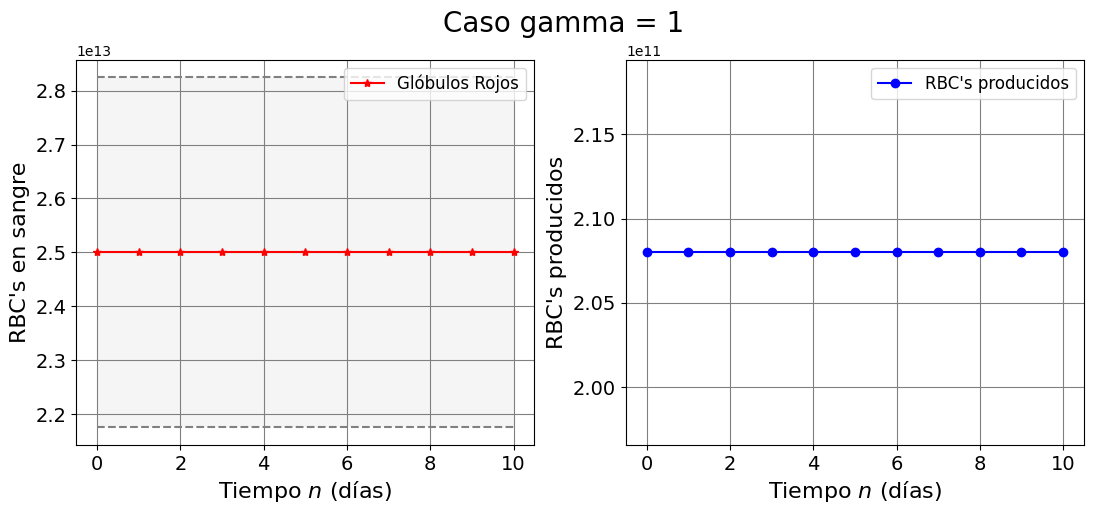
\includegraphics[scale=0.534]{BaseG1.png}
    \caption{Simulación del modelo para $\gamma = 1$. A la izquierda está la gráfica de $R(n)$, a la derecha la de $M(n)$.}
    \label{sec:modelo:fig:G1}
\end{figure}

Como era esperado, según los análisis hechos en la sección \ref{sec:modelo:analisis}, para el caso $\gamma = 1$ se obtiene una simulación totalmente estable, manteniendo el nivel de glóbulos rojos diarios en $25\times 10^{12}$ y la cantidad de glóbulos rojos producidos diariamente en $208\times 10^{9}$ como bien se puede observar en las gráficas de la figura \ref{sec:modelo:fig:G1}. Esta simulación representa el caso ideal en el que un paciente no tenga ninguna enfermedad o complicación médica y sea completamente saludable. Para este caso, todo glóbulo rojo que es eliminado por el bazo es producido por la médula ósea, por lo que no hay variaciones en las cantidades.

\subsection{Caso $\gamma=0.7$}
\begin{figure}[H]
    \centering
    \captionsetup{justification=centering}
    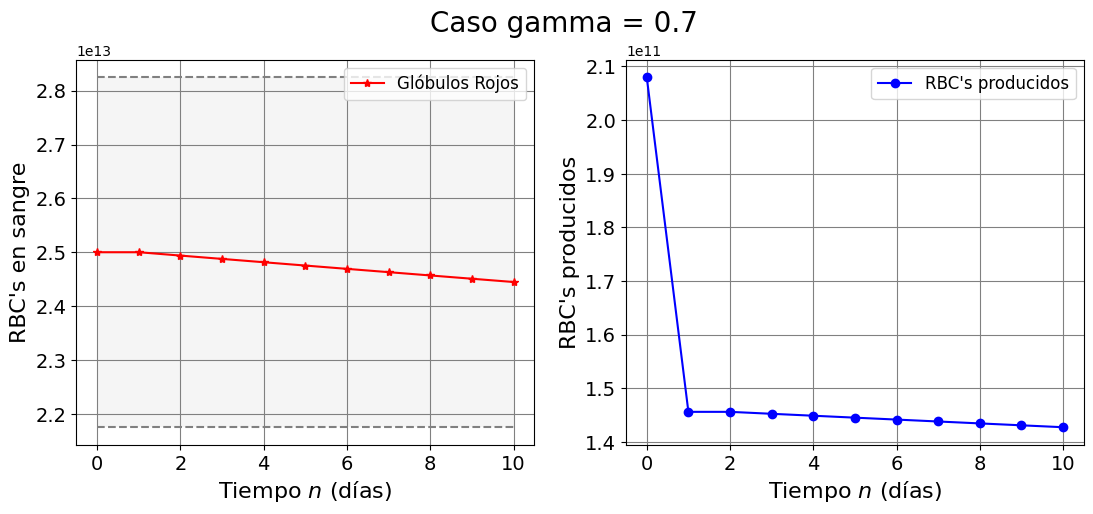
\includegraphics[scale=0.534]{BaseG07.png}
    \caption{Simulación del modelo para $\gamma = 0.7$. A la izquierda está la gráfica de $R(n)$, a la derecha la de $M(n)$.}
    \label{sec:modelo:fig:G07}
\end{figure}

En este caso, el paciente padece de una enfermedad que afecta la producción de glóbulos rojos producidos por la médula ósea, pues $\gamma=0.7$ implica que por cada glóbulo rojo eliminado por el bazo se producen únicamente $0.7$ glóbulos rojos. Como se puede observar en las gráficas de la figura \ref{sec:modelo:fig:G07}, los efectos de una baja producción de RBC's es una caída tanto en la cantidad de eritrocitos en el cuerpo como en su producción por parte de las células madre. Extendiendo los días simulados se encuentra que en el día 280 la cantidad de glóbulos rojos se ha reducido a la mitad respecto a la inicial. Un aspecto interesante es la caída que se puede observar en la segunda gráfica y la estabilidad en la primera del día 0 al día 1. Esta ocurre dado que las condiciones iniciales asumen que en el día 0 la producción es normal y a partir del día 1 es que ocurre el cambio en la producción de RBC's, por lo que ahí ocurre la primera caída en producción y en cantidad. 


\subsection{Caso $\gamma=1.3$}\label{subsec:modelo:simulaciones:G13}

En este caso, el paciente produce más glóbulos rojos de los que elimina. Esto puede tener diferentes causas, como bajos valores de hierro y, por lo tanto, de hemoglobina o dificultades pulmonares del paciente que produzcan bajos niveles de oxígeno en la sangre. Como bien se puede observar en las gráficas de la figura \ref{sec:modelo:fig:G13}, para valores de $\gamma$ mayores a 1 se obtiene un crecimiento en la cantidad de glóbulos rojos en el cuerpo y en la cantidad diaria producida por la médula ósea, esto se debe a que el cuerpo está produciendo una media de 1.3 RBC's por cada uno perdido, por lo que es normal que la cantidad de estos aumente. Así como en la simulación para $\gamma = 0.7$, la anomalía presentada del día 0 al día 1 se debe a las condiciones iniciales del problema. Al extender los días de la simulación, se encuentra que en el día 183 la cantidad de eritrocitos en el cuerpo se ha duplicado respecto al valor inicial. Como se analizó en la sección \ref{sec:modelo:analisis}, si se quisiera extender la simulación al infinito los glóbulos rojos también tenderían hacia el infinito. 

\begin{figure}[H]
    \centering
    \captionsetup{justification=centering}
    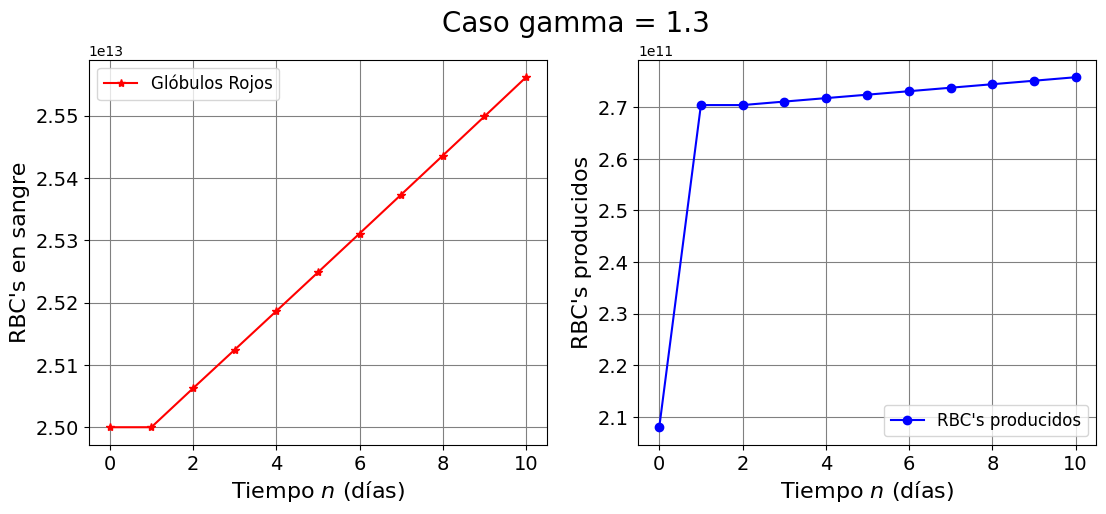
\includegraphics[scale=0.534]{BaseG13.png}
    \caption{Simulación del modelo para $\gamma = 1.3$. A la izquierda está la gráfica de $R(n)$, a la derecha la de $M(n)$.}
    \label{sec:modelo:fig:G13}
\end{figure}
Habiendo ya analizado y entendido el modelo base para los diferentes casos, el siguiente capítulo buscará acoplar a este modelo dos variaciones posibles: cuando el paciente padece anemia renal o cuando el paciente ha sufrido una hemorragia.